\documentclass{article}
\usepackage{graphicx} % Required for inserting images
\usepackage[T1]{fontenc}
\usepackage{amssymb, amsmath, graphicx, subfigure, enumitem}
\usepackage[top=1in, bottom=1in, left=1in, right=1in]{geometry}
\usepackage{fancyhdr}
\usepackage{hyperref}
\usepackage{xcolor}

\newenvironment{simplechar}{%
   \catcode`\$=12
   \catcode`\&=12
   \catcode`\#=12
   \catcode`\^=12
   \catcode`\_=12
   \catcode`\~=12
   \catcode`\%=12
}{}

\pagestyle{fancy}
\fancyhead{} % clear all header fields
\fancyfoot{} % clear all footer fields
\fancyhead[C]{}
\fancyfoot[C]{\thepage}

\title{Conformers Homework}
\author{Kevin Wang, Timber Lin, Theophilus Pedapolu}
\date{April 2023}

\begin{document}

\maketitle
\thispagestyle{plain}
\noindent
In this homework, we guide you through the Conformer, a novel deep-learning architecture that combines convolutional layers with transformers to capture both the local and global dependencies of an audio sequence. It has shown state-of-the-art results on automated speech recognition (ASR) tasks. The first 2 questions are analytical questions meant to help you understand a new convolution operation and activation function you may not have heard of but which are key components of the Conformer. The rest of the homework deals with implementing and training a conformer. The original Conformer paper is here: \href{https://arxiv.org/abs/2005.08100}{\color{blue}{https://arxiv.org/abs/2005.08100}} We encourage you to read through this paper before starting this homework.

\newpage
\thispagestyle{plain}
\section{Depthwise-Separable Convolutions}
So far, we have learned about the convolution operation in which we take a kernel and slide it over an input, multiplying element-wise and summing at each position to produce an output. Although convolutional layers require far fewer computations than FFN layers, there are cases when we would like to reduce the computation even further. This is the motivation behind depthwise-separable convolutions. These are a type of convolution that "separate" the standard convolution procedure into two parts: depthwise convolution and pointwise convolution. \newline\newline
Suppose we have a $M\times N\times D$ input tensor. In standard convolution, we would use $D$ kernels of size $K\times K \times D$ where $K$ is the kernel size and $C$ is the number of desired output channels. The output would then be of the form $M'\times N' \times C$  Notice that the depth of the kernel equals the depth of the input tensor. In depthwise convolution, however, we separate the depth dimension and instead have $D$ kernels of size $K\times K \times 1$. Each kernel is convolved separately at a different depth to produce outputs of shape $M' \times N' \times 1$. These outputs are then stacked to produce a tensor of shape $M'\times N' \times D$. Figure $1$ visually shows this procedure. 
\newline\newline
Pointwise convolution is then applied on the $M'\times N' \times D$ tensor to change $D$ to a desired number of channels $C$. The term "pointwise" refers to the fact that this type of convolution uses $C$ kernels of shape $1\times 1 \times D$. Each kernel is applied on the entire tensor to produce an output of shape $M'\times N' \times 1$. These outputs are again stacked in the channel dimension to produce a final $M'\times N' \times C$ tensor, the same shape we would get in standard convolution. As you can see depthwise-separable convolutions are very similar to standard convolutions, except that we selectively apply the kernels first to the 2D dimensions (M and N) then across the channel dimension (D) instead of all dimensions at once.

\begin{figure}[h]
  \centering
  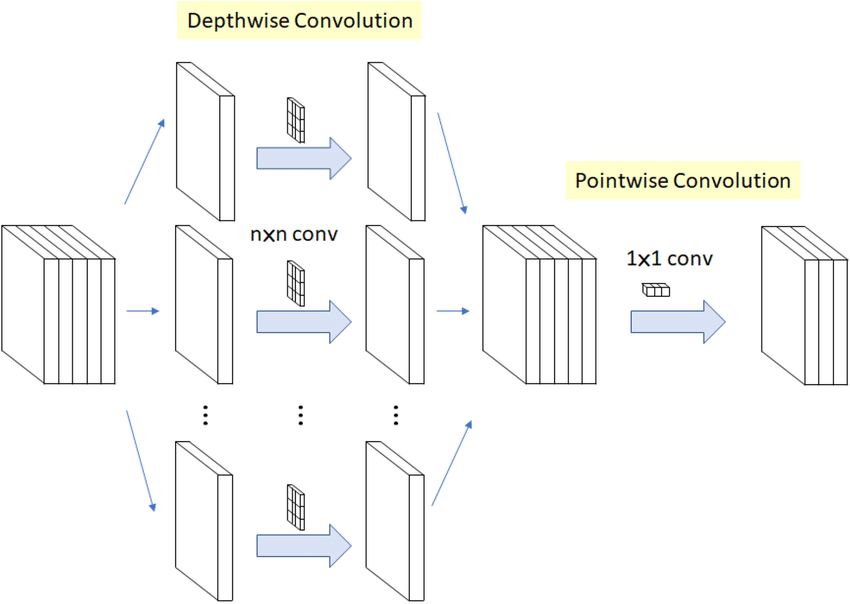
\includegraphics[scale=0.35]{Depthwise-Separable_Conv.png}
  \caption{Visual of how depthwise and pointwise convolutions are performed. Source: Analytics Vidhya}
  \label{fig:example}
\end{figure}

\newpage
\thispagestyle{plain}
\newgeometry{top=1in, bottom=1in, left=1in, right=1in}
Suppose we have the $3 \times 3 \times 3$ input tensor A below

\[ A = 
\begin{bmatrix}
    \begin{bmatrix}
        4 & 8 & 2 \\
        1 & 5 & 9 \\
        7 & 6 & 3
    \end{bmatrix}
    &
    \begin{bmatrix}
        0 & 4 & 6 \\
        9 & 7 & 5 \\
        3 & 8 & 1
    \end{bmatrix}
    &
    \begin{bmatrix}
        7 & 4 & 2 \\
        1 & 0 & 5 \\
        0 & 5 & 1
    \end{bmatrix}
\end{bmatrix}
\]
\newline\newline
 For subparts to this question, assume all convolutions are performed with stride = 1 and padding = 0

\begin{enumerate}[label=(\alph*)]
    \item Compute the depthwise convolution on A using the $2 \times 2 \times 1$ kernels below in order
    \[K_1 = 
        \begin{bmatrix}
        \begin{bmatrix}
            0 & 1 \\
            2 & 3
        \end{bmatrix}
        \end{bmatrix}
        \;\;\;
      K_2 = 
      \begin{bmatrix}
      \begin{bmatrix}
            4 & 5 \\
            0 & 9
        \end{bmatrix}
        \end{bmatrix}
        \;\;\;
      K_3 = 
      \begin{bmatrix}
      \begin{bmatrix}
            4 & 0 \\
            0 & 8
        \end{bmatrix}
        \end{bmatrix}
        \;\;\;  
    \]
    \item Perform pointwise convolution on the output you computed in part (a) using the $2 \times 2 \times 3$ kernels below in order. You should have 2 channels in the final output
    \[K_1 = 
        \begin{bmatrix}
        \begin{bmatrix}
            1
        \end{bmatrix}
        &
        \begin{bmatrix}
            0
        \end{bmatrix}
        &
        \begin{bmatrix}
            2
        \end{bmatrix}
        \end{bmatrix}
    \]
    \[K_2 = 
        \begin{bmatrix}
        \begin{bmatrix}
            4
        \end{bmatrix} 
        &
        \begin{bmatrix}
            1
        \end{bmatrix}
        &
        \begin{bmatrix}
            3
        \end{bmatrix}
        \end{bmatrix}
    \]
    \item In this example with the $3 \times 3 \times 3$ input tensor, how many different parameters were used for both the depthwise and pointwise convolution steps? Suppose we instead performed standard convolution with $2$ kernels of shape $2 \times 2 \times 3$ to get the same final output shape. How many parameters would we use in this case?

    \item Now we will use the number of multiplications performed as a proxy for computational cost. Again For the depthwise-separable convolution (depthwise and pointwise steps), how many total multiplications were performed. Ignore any addition operations involved in calculating sums. For standard convolution using the same kernels in the previous part, how many multiplications were performed?

    \item Consider the general case, where we have a $M \times N \times D$ input tensor. Suppose we use $K \times K \times 1$ kernels for depthwise convolution and $C$ kernels of size $1 \times 1\times D$ kernels for pointwise convolution. How many parameters are used in the depthwise-separable convolutional layer altogether? How many multiplications are performed? Calculate the parameters and multiplications for a standard convolutional layer as well assuming we use $C$ kernels of size $K \times K \times D$

    \item Using this information about the number of parameters and the number of multiplications performed, what can you say about the computational and memory efficiency of depthwise-separable convolutions vs. standard convolutions? Is one more efficient than the other?

    \item What are the benefits and drawbacks of depthwise-separable convolutional layers? Why don't we use them all the time?
\end{enumerate}

\newpage
\thispagestyle{plain}
\section{Understanding the Swish Activation Function}
The swish activation function is $y=\frac{x}{1+e^{-x}}$, and is sometimes called the sigmoid weighted linear unit. Some of its properties include: being bounded below but not above, non-monotonicity, and smoothness, and these in combination are believed to be advantageous. Although the swish function is inspired by the sigmoid activation function, the swish function critically avoids the vanishing gradient problem suffered by the sigmoid function. Meanwhile, the swish function is quite similar to the relu activation function but importantly has a smooth output which is likely less sensitive to initialization and learning rates, making it easier to optimize than with relu. The swish activation hopes to capture the advantages of both the sigmoid and relu activation functions and has seen better results in deeper networks.\newline\newline
(a) Show that the derivative of the swish activation function can be expressed as $y'=y+\sigma (x)*(1-y)$ where $\sigma (x)=\frac{1}{1+e^{-x}}$, and explain how this addresses the vanishing gradient problem that affects the sigmoid activation.\newline\newline
(b) How is the swish activation function similar to the self-gating component of the LSTM cell?\newline\newline
(c) There is a modified version of the swish activation function, which includes a tunable $\beta$ parameter: $z=\frac{x}{1+e^{-\beta x}}$. Show that the derivative of this modified swish activation function can be expressed as $z'=\sigma (\beta x)+\beta x \sigma (\beta x)*(1-\sigma (\beta x)) = \beta z + \sigma(\beta x) * (1-z)$\newline\newline
(d) Usually, the value of $\beta$ is near $1$. If we were to increase $\beta$ towards $\infty$, what activation function would the modified swish activation approach?\newline\newline
(e) Why would a $\beta$ value near 0 create issues?\newline\newline

\newpage
\thispagestyle{plain}
\section{Coding Question: Designing the Conformer Architecture}
Follow the instructions in this notebook and complete all the TODOs to build the different parts of the conformer and write the pipeline. Make sure you pass all the test cases: 
\href{https://colab.research.google.com/drive/1r5xv6N49ooYWbXL95672rZyXyFMNd3jL?usp=sharing}{\color{blue}{Conformers.ipynb}}

\newpage
\thispagestyle{plain}
\section{Training Conformers for ASR and Ablation Studies}
Run through the CoLab notebook \href{https://colab.research.google.com/drive/1h_ML3mGcVd3opaa2ctxL3ZnuI2LV1uyz?usp=sharing}{\color{blue}{Conformers\_ASR.ipynb}} and follow all the steps to train the Conformer models and plot losses. Note that some of the training may take up to 10-15 minutes and please make sure to use a GPU in your runtime. Include your answers to the written questions below
\newline
\begin{enumerate}[label=(\alph*)]
\item\mbox{}\\
\begin{enumerate}[label=(\roman*)]
    \item Experiment with the parameters used to create the Conformer encoder: \newline encoder\_dim, num\_encoder\_layers, depthwise\_conv\_kernel\_size. In general, does increasing or decreasing any of the parameters give better performance?

    \item Notice that the model takes in an argument called "input\_lengths," which contains the lengths of the non-padded sequences for elements in the batch. Why does the conformer encoder need this information? Which part of the pipeline is this most important for?

    \item What does the decoder consist of for this model? What is contained in the final outputs of the model?

    
\end{enumerate}
\item\mbox{}\\ 
\begin{enumerate}[label=(\roman*)]
    \item How does increasing the number of heads in the conformer encoder influence the performance, i.e. the loss rates? Can you give an intuitive explanation as to why?
    
    \item In language prediction, multiple heads capture different dependencies in the input text such as subject-verb relationships and pronoun references. What is the audio analog of this idea? In other words, what kind of information do the different heads capture about the audio signal?

    
\end{enumerate}
\item\mbox{}\\
\begin{enumerate}[label=(\roman*)]
    \item Did one model perform better than the other, either the one with the convolution module first or the one with the self-attention module first?

    \item In the original paper, the authors also tried to split the input into parallel branches of a multi-headed self attention module and a convolution module with their output concatenated, which yielded worse performance. What does this tell you about the best architectural design for the Conformer block?

\end{enumerate}
\end{enumerate}

\newpage
\thispagestyle{plain}
\section{Homework Process and Study Group}
\begin{enumerate}[label=(\alph*)]
    \item What sources (if any) did you use as you worked through the homework?
    \item If you worked with someone on this homework, who did you work with?
        List names and student ID’s. (In case of homework party, you can also just describe the group.)
    \item Roughly how many total hours did you work on this homework? Write it down here where you’ll need to remember it for the self-grade form.

\end{enumerate}

\newpage
\thispagestyle{plain}
\section{References}
[1] Gulati, Anmol, et al. "Conformer: Convolution-augmented transformer for speech recognition." arXiv preprint arXiv:2005.08100 (2020). 
\newline\newline
[2] Ramachandran, Prajit, Barret Zoph, and Quoc V. Le. "Searching for activation functions." arXiv preprint arXiv:1710.05941 (2017)
\newline\newline
[3] Kaiser, Lukasz, Aidan N. Gomez, and Francois Chollet. "Depthwise separable convolutions for neural machine translation." arXiv preprint arXiv:1706.03059 (2017).
\end{document}
